\documentclass[a4paper,11pt]{article}

\usepackage[utf8]{inputenc}
\usepackage[american]{babel}
\usepackage{csquotes}
\usepackage[style=apa]{biblatex}
\usepackage{graphicx}
\usepackage{float}

\bibliography{project-specification}

\graphicspath{{images/}}

\begin{document}

\title{FIT3036 --- Project Specification}
\author{Dylan Pinn --- 24160547}
\maketitle
\pagebreak

\tableofcontents
\pagebreak

\section{Introduction}

% TODO: Improve introduction

This project specification outlines the plan to design, implement, test and
deliver the FIT3036 Computer Science project.

Go through

project requirements
project plan
external design
Internal design
software architecture
test plan

\section{Project Requirements}

The functional and non-functional requirements of the project have been outlined
in the following sections.

\subsection{Functional Requirements}

The functional requirements are:

\begin{itemize}
  \item System shall allow a user to select a 1 square km area on Google Maps.
  \item System shall allow a user to request the total area of the roads within
    the nominated square area.
\end{itemize}

\subsection{Non-functional Requirements}

The non-functional requirements are:

\begin{itemize}
  \item System shall be easily accessible via the Internet.
  \item System shall be testable.
  \item System shall be affordable to host.
  \item System shall be easy to deploy.
  \item System shall be easy to maintain.
  \item System shall be well documented.
\end{itemize}

\section{Project Plan}

% TODO: Add section introduction

3. Project Plan
  1. Overview - Project objectives, requirements and constraints.
  2. Risk Analysis - What are the main project risks, their probabilities and risk reduction strategies?
  3. Resource Requirements - Hardware and software (more specific than Functional Requirements)
  4. Schedule - Corresponding to tasks identified above (e.g. in a Gantt chart, PERT chart, Kanban, etc...)


\subsection{Overview}

% TODO: Improve Overview

\paragraph{Project Objectives:}

Our company secured a contract for a local council in Victoria to re-surface
roads in a designated kilometre area. The objectives are to design, implement,
test and deliver a system that will perform these calculations and display the
result to the user.

\paragraph{Requirements:}

We are to use Google Maps and related products and any satellite/aerial views.
The project involves writing the related code, with an elegant GUI to support
calculations.

% TODO: Add citation to online pdf for Project Intro
% \autocite[1]{INTRO:1}

\paragraph{Constraints:}

We have the following constraints on the project:

\begin{itemize}
  \item Only have access to publicly available data.
  \item Limited to available information online.
  \item No / Limited access to council records.
  \item Project must be finalised by the end of week 12.
\end{itemize}

\subsection{Risk Analysis}

% TODO: Attach Google Docs sheet and expand

Done some risks in attached document. Need to expand and add more if time permits.

\subsection{Resource Requirements}

\paragraph{Hardware:}

We have decided to use as much Software as a Service (SaaS), Platform as a
Service (PaaS) and Infrastructure as a Service (IaaS) solutions to keep costs
down.

Amazon Web Services (AWS) has been chosen to use due to its comprehensive free
tier and prior experience with the platform. The following AWS services are
going to be utilised:

\begin{itemize}
  \item AWS Lambda --- Functions as service; allows running back-end code without
    maintaining server infrastructure.
  \item AWS API Gateway --- Allows creating public API endpoints for Lambda
    functions
  \item AWS S3 --- Cheap scalable storage to store front-end code.
  \item AWS Cloudfront --- CDN for front-end code. Speeds up delivery by caching
    content.
  \item AWS Cloudformation --- Service to provision services on AWS.\@
\end{itemize}

We are going to use continuous integration and continuous deployment using
Travis which offers free plans for Open Source software. This allows us to use
the latest devops practices to automate running tests and deploying the latest
tested code.

\paragraph{Software:}

The following is an outline of the software required for the project:

\begin{itemize}
  \item Local development environment --- Code editor, IDE, terminal, etc.
  \item NodeJS --- Required to build front-end code.
  \item Go Programming Language --- Required to build back-end code.
  \item \LaTeX{} --- Required to build documentation.
\end{itemize}

\subsection{Schedule}

% TODO: Finalise schedule

Created a Gantt Chart, as seen in figure \ref{fig:gantt}, from our Trello board using TeamGantt. This allows working back from the due date to meet deadlines.

\begin{figure}[H]
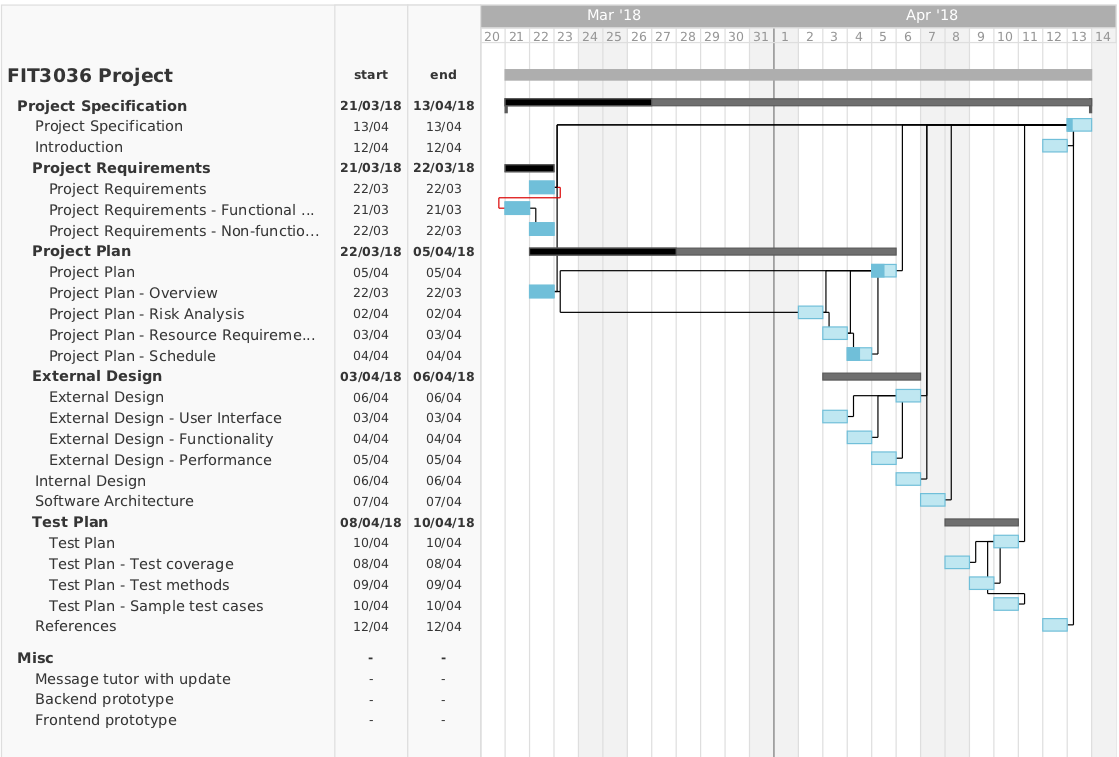
\includegraphics[width=\textwidth]{gantt-chart}
\caption{Gantt chart}
    \label{fig:gantt}
\end{figure}


\section{External Design}

% TODO: Add section introduction

4. External Design - Externally observable features of your simulation: input, output, performance.
  1. User Interface - How to run the software
  2. Functionality - Any externally available functions not covered above.
  3. Performance - Time and space performance characteristics of your software.


\subsection{User Interface}

% TODO: Finalise User interface

Created mockup figure \ref{fig:mockup}. %TODO: Add square to mockup.

Open webpage and presented with a large render of Google Maps. There is a square that can be positioned and sized over the map for the user to select the area to calculate.

A calculation shows the total area of the shape over the map.

The user then pushes the "Calculate" button to generate the surface area of the roads within the square.

There is help information on the page.

\begin{figure}[H]
  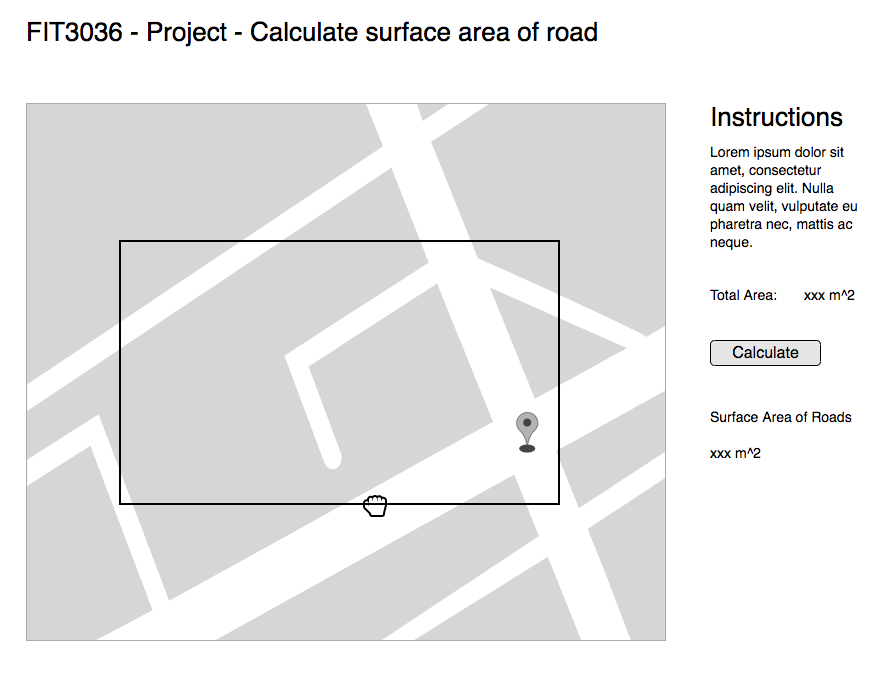
\includegraphics[width=\textwidth]{UI-mockup}
  \caption{Application Mockup}
  \label{fig:mockup}
\end{figure}

\subsection{Functionality}

% TODO: Finalise functionality

API will be created that will take 4 position parameters, each boundary is made up of a Latitude and Longitude.

This method calls the Open Street Maps API with these params to return all of the streets within the boundaries.

This is then passed to a method that will use the Haversine distance calculation to calculate distance between all of the nodes. If lane information is provided then this is multiplied by by the default lane length (3.5m) if not then the default is used. (NEED TO CHECK IF HAS MULTIPLE LANES). This is then summed and returned.

Lane width 3.5m https://www.driverknowledgetests.com/resources/road-widths/

%Haversine formula https://en.wikipedia.org/wiki/Haversine_formula

Another API is exposed for the frontend UI.

It takes 4 position parameters, each with boundary is made up of a Latitude and Longitude. This will calculate the total area of the 4 points and return it.

Calculate the area of 4 points:
%http://mathforum.org/library/drmath/view/63767.html

\subsection{Performance}

% TODO: Finalise Performance

Time:
We would like the response from the API to calculate the area of the square to be very fast (< 0.5s) as this will run whenever, the area is changed.

The main method that will calculate the total surface area of the all of the roads will also need to be sum what fast as we don't want the user to have to wait a long time while this is calculated. < 1m

Space:
AWS Lambda, which is where the backend code is run, can run between 128MB-3008MB memory to run the method. The default is 1024MB which is what I will be using.


\section{Internal Design}

5. Internal Design - Description of how the software is meant to work together (e.g. ‘the harvester module dumps data to the data logging module’…; illustrate with use cases or sequence diagrams)

% TODO: Finalise internal design
% TODO: Add sequence diagrams

Calculate Total Surface Area:

User drags or resizes square in Map.
These params are sent to the backend service
This calculates the total surface area
This is returned to the user
Calculate Total Surface Area of Roads in Area:

User requests to calculate total surface area
Params are sent to calculateSurfaceAreaofRoads
These are used to call OpenStreetMap API
Iterate over data and call calculateDistance
pass response to addLaneWidth
result summed
return to user


\section{Software Architecture}

6. Software Architecture - Overall structure of the code; high-level class structure (if any, e.g. via UML class diagrams …)


% TODO: Finalise Software Architecture
% TODO: Add class diagram

Classes made up of methods that help calculate the areas.

\section{Test Plan}

7. Test Plan
  1. Test coverage - Test coverage in the test plan states what requirements will be verified during what stages of the product life. (e.g. JUnit testing during phase X…)
  2. Test methods - Test methods in the test plan state how test coverage will be implemented (e.g. unit testing, acceptance testing, ...)
  3. Sample Test Cases - what data will be collected, and how that data will be stored and reported. One outcome of a successful test plan should be a record or report of the verification of all design specifications and requirements as agreed upon by all parties.

% TODO: Add section introduction

Test Plan

1. Test coverage - Test coverage in the test plan states what requirements will be verified during what stages of the product life. (e.g. JUnit testing during phase X…)
2. Test methods - Test methods in the test plan state how test coverage will be implemented (e.g. unit testing, acceptance testing, ...)
3. Sample Test Cases - what data will be collected, and how that data will be stored and reported. One outcome of a successful test plan should be a record or report of the verification of all design specifications and requirements as agreed upon by all parties.

\subsection{Test coverage}

% TODO: Finalise test coverage

Use jest and react-testing-library for testing frontend components.

Use Go inbuilt testing package for unit testing backend classes, functions.

These will automatically be run through development using tools to test runners.

Tests will be run automatically through CI/CD service before deploying changes to ensure that functionality is enforced.

\subsection{Test methods}

% TODO: Finalise test methods

Unit tests on all class methods. This verifies that the individual functions behave as expected.

Integration tests for API backends to ensure that correct response is returned for known parameters.

Unit test frontend components to ensure that they behave and interact in the correct manor.

Acceptance testing to make sure requirements are met.

Able to generate test coverage reports for front end and back end code. 80-100% test coverage is acceptable.

System tests will test the system as a whole and test the entire functionality.


\subsection{Sample test cases}

% TODO: Finalise sample test cases

Test plan

Test a known Area to calculate the total area.
Test a known Distance to know the length of it.
Test a known Area to sanity check the surface area of the roads within it.

% TODO: Put on new page

\pagebreak

\section{References}

%\printbibliography

8. References – References need to be provided in a correct and consistent format. Use BibTeX, EndNote, etc. to help in generating a correct list of references.

% TODO: Finalise references
% TODO: Generate reference file. Check against Monash IT reference style.

Collate references from workbook entries

React, NodeJS, Jest, React Testing Library, Go Lang, Go Testing Package.

Open Street Maps.
Default Lane width.

%https://www.pmi.org/learning/library/risk-analysis-project-management-7070

AWS services

Latex

CI/CD - Travis

\end{document}
